\section{Graphs in the finite upper half plane}
After passing by the representation theory of groups we can try to apply it to the study of some kinds of graphs constructed
over the finite upper half plane. There is a nice connection between the ideas above and the complex Poincaré upper half plane. We
do not have enough space to deal with it. See for instance \cite{terras_1999}.

Now we start with main definitions and proofs.
\subsection{The finite upper half plane}
\begin{defn}
	An element $\gamma \in \F_q$ is a {\it square} if $\exists \, x \in \F_q \colon \gamma = x^2$.
\end{defn}
If $\delta$ is a non square element of $\F_q$, then the polynomial $x^2 - \delta$ has no solutions in $\F_q$.
Its splitting field is $\F_{q^2}$ and one of its roots will be denoted by $\rd$ (the other is $-\rd$). 

$\rd$ will play the same role of the imaginary unit $i$. Given $z=x+y\rd \in \F_{q^2}$ we define,
using the notation from complex analysis, the {\it real part} of $z$ as $\Re z = x$;
the {\it imaginary part} of $z$ as $\Im z = y$;
the {\it conjugate} of $z$ as $\bar{z} = x-y\rd$; the {\it norm} of $z$ as $\Norm z = z \, \bar{z}$;
the {\it trace} of $z$ as $\Trace z = z+\bar{z}$.
\begin{rem}
The norm and the trace above are the ones usually defined in theory of finite fields (in the special case of the field 
extension $\F_{q^2}$ over $\F_q$), because $z^q= (x+y\rd)^q = x^q+y^q \rd^q = x+y(-\rd) =\bar{z}$.
See for instance \cite{lidl1994introduction}.
\end{rem}
\begin{defn}
	The {\it finite upper half plane} is
	\begin{equation}
		H_q = \big\{ z=x+y \rd \colon x \in \F_q,\, y \in \F_q^* \big\} 
	\end{equation} 
\end{defn}

We recall the definition of group action.
\begin{defn}
  A {\it group action} of the group $G$ on the set $X$ is a map
  \begin{align*}
	\phi \colon H \times X & \longrightarrow X \\ (g,x) &\longmapsto \phi (g,x) = g \cdot x
\end{align*}
such that:
\begin{itemize}
\item $\forall \, x \in X,\, \iota \cdot x = x$, where $\iota$ denotes the identity of the group;
\item $\forall \, h,g \in G, \forall\, x \in X$ we have $(gh)\cdot x=g \cdot (h\cdot x)$.
\end{itemize} 
\end{defn}

In our case will have $X=H_q$, while $G$ will be the general linear group $\GL(2,\F_q)$ or its subgroup of
affine transformations $\Aff (q)$.

Now we can define define the action we are interested in, and investigate some of its properties.
\begin{defn}\label{flt}
The group $\GL(2,\F_q)$ acts on $H_q$ by {\it fractional linear transformation}:
\begin{equation}
	\forall g= \begin{pmatrix} a & b \\ c & d \end{pmatrix}\in \GL(2,\F_q),\, \forall z \in H_q, \quad g \cdot z = \frac{az+b}{cz+d}.
\end{equation}
\end{defn}

We check the well definition of the action and find some properties in the following proposition.

\begin{prop}
Given $\cdot$ the action by fractional linear transformation, the following holds (with the same notations of \ref{flt}):
\begin{itemize}
\item[1.] $\Im (g\cdot z) = \frac{\Im z \det g}{\Norm (cz+d)}$ and
$\Re (g\cdot z) = \frac{ac\Norm z +bd+(ad+bc)\Re z}{\Norm (cz+d)}$;
\item[2.] the action is well defined;
\item[3.] the restriction of of the action to the subgroup $\Aff (q)$ is a {\it transitive} action, that is:
	$\exists \, \bar{z} \in H_q \colon \big( \forall z \in H_q\, \exists g \in \Aff (q)\,\,\text{such that}\,\, z=g \cdot \bar{z} \big) $. 
\end{itemize}
\begin{proof}
To prove 1. we have to show first that $\Norm (cz+d)\neq 0$. 
By definition of norm it suffices to prove that $cz+d \neq 0$  Let $z=x+y\rd$. Then
\begin{equation}\label{den}
	cz+d=0 \iff (cx+d)+(cy)\rd=0 \iff cy=0 \land cx+d=0 \iff c=d=0,
\end{equation}
but this cannot happen, because $\det g = ad-bc \neq 0$. Then is enough to write down the definition of $g\cdot z$.

Now we prove the second part. We already proved that $cz+d\neq 0$ in \ref{den}.
We have now to show that $g\cdot z \in H_q$, that is $\Im (g\cdot z)\neq 0$. But this follows from point 1:
$\Im (g\cdot z) = \frac{\Im z \det g}{\Norm (cz+d)}$, where $\Im z \neq 0$ because $z \in H_q$,
$\det g \neq 0$ because $g \in \GL(2,\F_q)$. The only thing left is to show that
$\forall \, h,g \in \GL(2,\F_q), \forall\, z \in H_q$ we have $(gh)\cdot z=g \cdot (h\cdot z)$, but this follows simply 
writing the definition of the action and the matrix product.

For the last part, take $\bar{z} = \rd \in H_q$. Then for any $z=x+y\rd \in H_q$ we have that $\begin{pmatrix} y & x \\ 0 & 1 \end{pmatrix} \cdot \bar{z} = z$ (note that $y\neq 0$ because $z \in H_q$, so the matrix defined belongs to $\Aff (q)$).
\end{proof}
\end{prop}
\begin{rem}
$\Aff q$ is a subgroup of $\GL(2,\F_q)$, so the action of $\GL(2,\F_q)$ is transitive too.
\end{rem}

Now we can introduce a {\it distance} (which is analogous to the arch length in the Poincaré upper half plane).
\begin{defn}
	The {\it distance} of two elements of $H_q$ is defined by:
	\begin{align*}
	\dist \colon H_q \times H_q & \longrightarrow H_q \\ (z,w) & \longmapsto \dist (z,w)= \frac{\Norm (z-w)}{\Im z \Im w}= \frac{(x-u)^2-\delta (y-u)^2}{yu},
\end{align*}
where $z=x+y\rd$ and $w=u+v\rd$ (the definition is well posed because $z,w \in H_q \Rightarrow y,v \neq 0$).
\end{defn}
\begin{rem}
The {\it distance} defined above is not a {\it metric}, that is its image is in $\F_q$ and not in $\R$. No triangle inequality is possible. The only properties of metric we have are: 
\begin{itemize}
\item [1.] $\dist (z,w)=\dist (w,z)$;
\item [2.] $\dist (z,w) =0 \iff z=w$.
\end{itemize}
\begin{proof}
The first item is trivial by definition, while the second one requires more care.

If $z=w$ then $x=u \land y=v$, so $\dist (z,w) =0$.

If $\dist (z,w) =0$ then $(x-u)^2-\delta (y-v)^2=0 \Rightarrow (x-u)^2 = \delta (y-v)^2$.
If $y-v\neq 0$ then $\delta = ((x-u)(y-v)^{-1})^2$, but this is impossible because $\delta$ is a non square element.
So $y=v$, which implies $x=u$ and $z=w$.
\end{proof}
\end{rem}

We are interested in this distance because it is invariant under the action of the group $\GL(2,\F_q)$ on $H_q$.
\begin{prop}
Given $g \in \GL(2,\F_q)$ and $z,w \in H_q$, we have that $\dist (z,w)=\dist(g \cdot z,g\cdot w)$,
where $\cdot$ is the action by fractal linear transformation.
\begin{proof}
We first notice a property of the norm. Let $z\in H_q$, $a\in \F_q$. Then
\begin{equation}\label{norm_prop}
\Norm (az) = az \, \overline{az} = az\bar{a}\bar{z}=aza\bar{z}=a^2 z \bar{z}=a^2 \Norm z.
\end{equation}
Moreover, we recall that if $z,w \in \F_{q^2}^{*}$, then $\Norm (z\,w)= \Norm z \Norm w$.
Now we can prove the proposition. With the usual notation
	\begin{align*}
	\dist (g\cdot z,g\cdot w)&=\frac{\Norm (g\cdot z-g\cdot w)}{\Im (g\cdot z) \Im (g\cdot w)}
							  =\frac{\Norm(\frac{az+b}{cz+d} -
							   \frac{aw+b}{cw+d})}{\frac{\Im z \det g}{\Norm (cz+d)}\frac{\Im w \det g}{\Norm (cw+d)}}=\\
							  &=\frac{\frac{\Norm\big((az+b)(cw+d)-(aw+b)(cz+d)\big)}{\Norm(cz+d)\Norm (cw+d)}}
							  {\frac{\Im z \Im w (\det g)^2}{\Norm (cz+d)\Norm (cw+d)}}
							  =\frac{\Norm \big((z-w)(ad-bc)\big)}{\Im z \Im w (\det g)^2}=\\
							  &=\frac{(\det g)^2 \Norm (z-w)}{\Im z \Im w (\det g)^2}=\dist (z,w).
	\end{align*}
%We can prove the proposition in the case $z=\rd$, because the action is transitive: let $h$ be such that
%$h \cdot \rd = z$. Then $g^{'} \cdot z = g^{'} h \cdot \rd = g \cdot \rd$, where $g=g^{'} h$, and
%$g^{'} \cdot w^{'} = g^{'} h h^{-1} \cdot w^{'} = g^{'} h \cdot (h^{-1} \cdot w^{'})= g \cdot w$, where $w= h^{-1} \cdot w^{'}$.
\end{proof}
\end{prop}

\subsection{Graphs and their properties}
Now we can finally introduce the graphs we are interested in.
\begin{defn}
 Fix $0\neq a\in \F_q$. The graph $\xq a$ is defined with vertexes the elements of $H_q$,
 and with edges the pairs of vertexes $z,w\in H_q$ such that $\dist (z,w) = a$.
\end{defn}
\begin{rem}
We notice that the graph is undirected because $\dist (z,w) = \dist (w,z)$.
\end{rem}

We performed some calculations using MAGMA and plot the graphs with SAGE to have the feeling of the properties of the
graphs we defined.

\begin{table}\centering
\begin{tabular}{|c|c|c|c|c|c| p{4.2cm} |}
\hline
$q$ & $\delta$ & $a$ & girth & diameter & degree & eigenvalues with multiplicity \\
\hline
3 & 2 & 1 & 3 & 2 & 4 & <-2, 2>, <4, 1>, <0, 3>\\
5 & 2 & 1 & 3 & 3 & 6 & <1, 4>, <-2, 5>, <6, 1>, <-3, 4>, <2, 6>\\
5 & 2 & 2 & 3 & 3 & 6 & <1, 4>, <6, 1>, <-2, 11>, <3, 4>\\
5 & 2 & 4 & 4 & 2 & 6 & <6, 1>, <0, 10>, <-4, 4>, <2, 5>\\
7 & 2 & 2 & 5 & 4 & 4 & <1, 2>, <3, 2>, <4, 1>, <0, 7>\\
7 & 3 & 1 & 4 & 3 & 8 & <-4, 7>, <2, 22>, <8, 1>\\
9 & $F.1^3$ & 1 & 3 & 4 & 10 & <2, 9>, <-2, 10>, <10, 1>\\
9 & $F.1^7$ & 2 & 3 & 4 & 10 & <2, 9>, <-2, 10>, <10, 1>\\
49 & $F.1^13$ & $F.1$ & 3 & 4 & 50 & <8, 50>, <-4, 50>, <10, 50>, <-6, 100>, <2, 49>, <50, 1>\\
\hline
\end{tabular}
\caption{Principal characteristics of the graph for soma values of $q$, $\delta$ and $a$.}\label{tab}
\end{table}
The degree in the table stands for the degree of an arbitrary vertex, since the graphs are (experimentally, for now) regular.
Looking at table \ref{tab} that we computed we can see that in all the cases that the graph is $q+1$ regular except for
one row (the first with $q=7$). But this happened because there is an error: 2 is a square in $\F_7$, so it is not of our interest.

We computed more values, and we find that the degree and the girth never exceed 4. We weren't able to prove this, but we found
a reference \cite{ANGEL199662} where this fact is proved. We will not explain the proof for reason of space.

Moreover we see that all the eigenvalues satisfy the Ramanujan bound, that is in our case $\vert \lambda \vert \le 2\sqrt{q}$.
We will analyze the spectra of the graph, even if in an incomplete way, and we will prove that all the one dimensional
eigenvalues satisfy this bound. Anyway this bound holds for all eigenvalues (as shown in \cite{terras_1999}),
but prove this would require other 30 pages in the report.

In figures \ref{fig1} and \ref{fig2} we put as an example the  plot of two of the graph of table \ref{tab} (${\text{X}}_3(2,1)$ and ${\text{X}}_5(2,2)$, but we actually plotted all of them). SAGE can plot graphs in different layouts, arranging vertices in different ways, so we exploited this possibility.

\begin{figure}[!htbp]
\centering
\hspace*{-1.5cm}
%\begin{subfigure}[b]{0.4\linewidth}
\subfloat[][Default layout]
{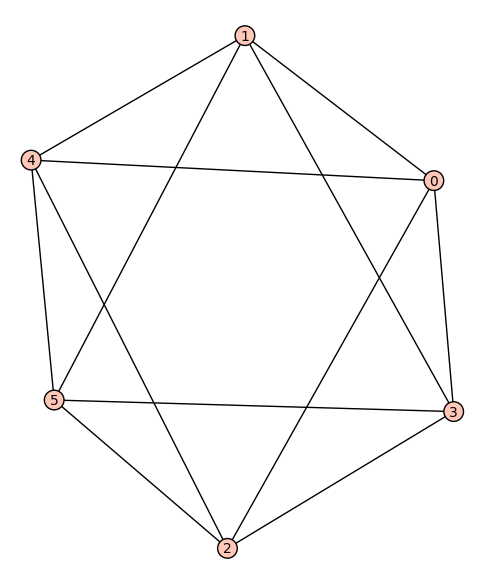
\includegraphics[width=0.4\linewidth]{q3}}
%\caption{Generic layout}
%\end{subfigure}%
%\begin{subfigure}[b]{0.4\linewidth}
\subfloat[][Planar layout]
{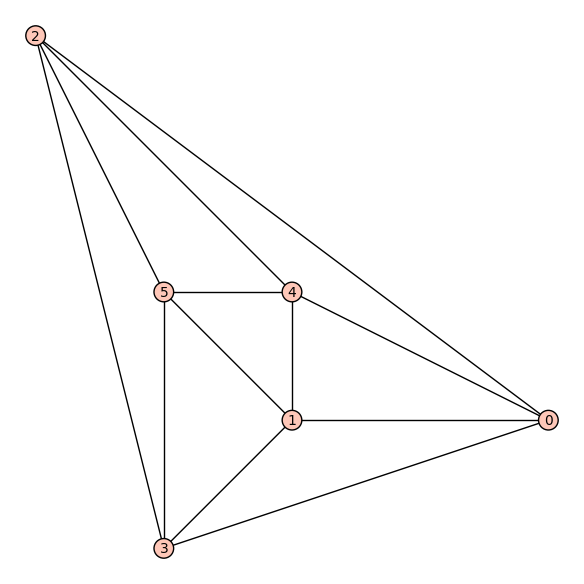
\includegraphics[width=0.4\linewidth]{q3_planar}}
%\caption{Planar layout}
%\end{subfigure}%
%\begin{subfigure}[b]{0.4\linewidth}
\subfloat[][Circular layout]
{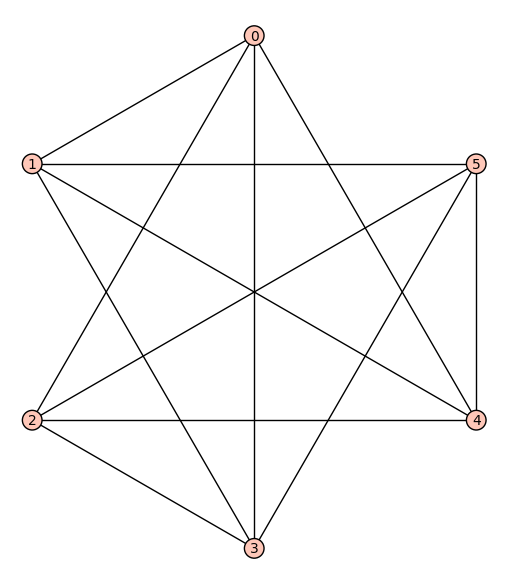
\includegraphics[width=0.4\linewidth]{q3_circularr}}
%\caption{Circular layout}
%\end{subfigure}
\caption{Different layouts for ${\text{X}}_3(2,1)$}
\label{fig1}
\end{figure}
\begin{figure}[!h]
\centering
%\hspace*{-1.5cm}
%\begin{subfigure}[b]{0.5\linewidth}
\subfloat[][Default layout]
{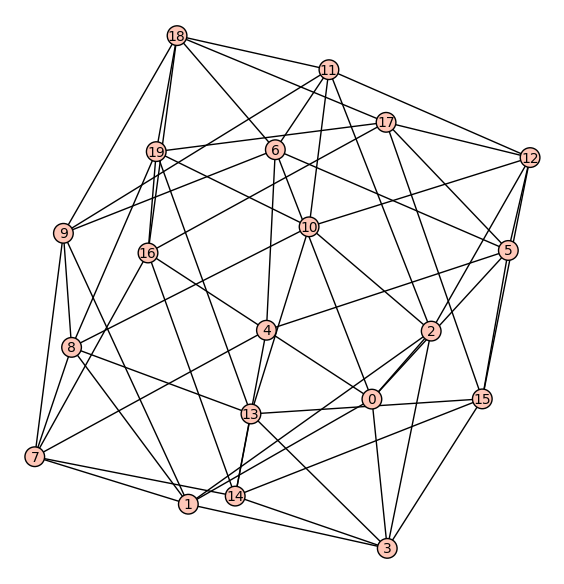
\includegraphics[width=0.45\linewidth]{q5_a2_d2}}
%\caption{Default layout}
%\end{subfigure}%
%\begin{subfigure}[b]{0.45\linewidth}
\subfloat[][Circular layout]
{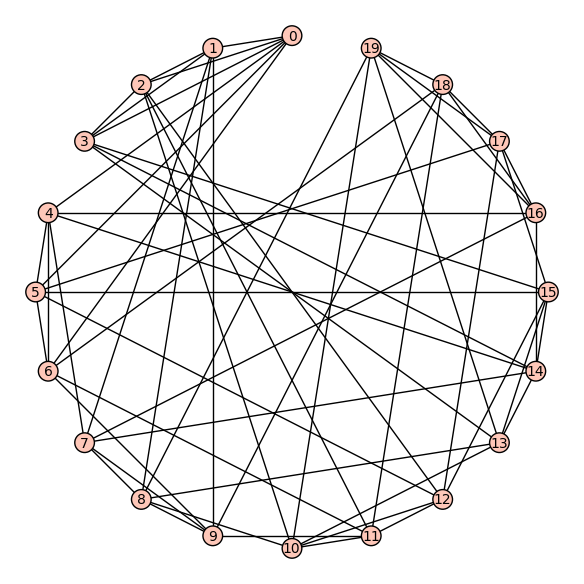
\includegraphics[width=0.45\linewidth]{q5_a2_d2_circular}}
%\caption{Circular layout}
%\end{subfigure}%
\caption{Different layouts for ${\text{X}}_5(2,2)$}
\label{fig2}
\end{figure}
%(qui ci vanno gli esempi, sia ripresi dal libro che no)
%(ci sono altre osservazioni carine sulle similutini col caso continuo, ma dovrei studiarci bene e non so se c'è spazio)
We can now state and prove one of the main theorems of the report.

\begin{theorem}\label{important}
Let $q=p^r$ , where $p$ is an odd prime. Let $0\neq a\in \F_q$, and let $\delta \in \F_q$ be a non square element.
Then the following holds:
\begin{itemize}
\item[1.] if $a\neq 4\delta$ then the graph is $(q+1)-regular$;
\item[2.] if $0\neq c\in \F_q$ then the graphs $\xq a$ and $X_q(\delta c^2, a c^2)$ are isomorphic;  
\item[3.] $\forall 0 \leq s < r, s\in \N$ the graphs $\xq a$ and $X_q (\delta^{p^s}, a^{p^s})$ are isomorphic;
\item[4.] if $a\neq 4\delta$ then $\xq a$ is the Cayley graph for the group $\Aff q$ with generators:
\begin{equation}\label{generators}
	S_q(\delta,a) = \Big\{ \begin{pmatrix} y & x \\ 0 & 1 \end{pmatrix} \in \Aff q \colon x^2=ay+(y-1)^2 \delta \Big\};
\end{equation}
\item[5.] if $a\neq 4\delta$ then $\xq a$ is connected.
\end{itemize}
\begin{proof}
1. WLOG I can assume $z=\rd$, because of the transitivity of the action and the invariance of the distance.
In fact, if $g \cdot \rd = z$, then 
\begin{equation*}
\lvert \{\bar{w} \colon \dist (\rd, \bar{w})=a\}\rvert=\lvert \{w \colon \dist (z,w)=a \} \rvert.
\end{equation*}
So we are interested in the solutions of the equation $\dist (\rd, z)=a$.

Suppose $z=x+y\rd$. Then
\begin{align} \label{distance}
	\dist (\rd, z)=a & \iff \Norm (\rd - z) = ay
					  \iff (\rd - z)\overline{(\rd - z)}=ay\\ \notag
					 & \iff (-x+(1-y)\rd)(-x-(1-y)\rd )=ay
					  \iff x^2 = ay + (y-1)^2 \delta. \notag
\end{align}
We must be careful: if $z$ is a solution of the previous equation, we must check that $z\in H_q$, that is $y\neq 0$.
But this is always true: if $y=0$ from the previous equation we obtain $\delta=(x(y-1)^{-1})^2$,
but this is impossible, since $\delta$ is a non square element.
So we can simply find solutions of $\Norm (\rd - z) = ay$ in $\F_{q^2}$, and they will belong to $H_q$ as well.

We recall (see \cite{lidl1994introduction}) that $\mathfrak{N}\colon \F_{q^2}^{*} \to \F_q^{*}$ is an onto group omomorphism.
We want to use this property to find the number of solutions of $\Norm (\rd - z) = ay$:
\begin{equation}
	\lvert \mathfrak{N}^{-1}(a)\rvert=\frac{\abs {\F_{q^2}^{*}}}{\abs {\F_q^{*}}}=\frac{q^2+1}{q-1}=q+1.
\end{equation}
Fix $c=(\frac{a}{2\delta}-1)\rd$ and $d=(1-\frac{a}{4\delta})a$. Then:
\begin{align*}
	\Norm (z+c) = d &\iff (z+c)(\bar{z}+\bar{c})=d \\
					&\iff ((z-\rd)+\frac{a}{2\delta})((\bar{z}+\rd)-\frac{a}{2\delta})=(1-\frac{a}{4\delta})a \\
					&\iff (z-\rd)(\bar{z}+\rd)+(\frac{a}{2\delta})(\bar{z}+\delta-z+\delta)+\frac{a^2}{4\delta}=a-\frac{a^2}{4\delta} \\
					&\iff \Norm (z-\rd)+(\frac{a}{2\delta})(-2y\rd +2\rd)=a \iff \Norm (z - \rd) = ay.
\end{align*}
So, if we set $w=z+c$, in the case $d\neq 0$, I can find $q+1$ solutions in $\F_{q^2}^{*}$ of $\Norm w = d$.
But $d=0 \iff a=0,4\delta$, cases that are excluded by hypothesis.

Hence the equation $\dist (\rd, z)=a$ has exactly $q+1$ solutions, that is the graph is $(q+1)-regular$.

2. We first notice that that $\delta c^2$ is a non square element, so the definition of the graph $X_q(\delta c^2, a c^2)$
is well posed. Clearly multiplying by $c^2$ is a bijection of $H_q$ to itself, so the vertexes of the two graphs are the same.

In the definition of $\Norm z = z \bar{z}$ seems that the choice of $\rd$ matters; but as we already noticed $\bar{z}=z^q$.
This means that $\Norm z = z z^q$ is independent from the choice of $\rd$. The same does not hold for the imaginary part:
if $z=x+y\rd$, then $z=x+yc^{-1} c \rd $. So, with an obvious notation, 
\begin{equation} \label{ims}
	\Im_{c\rd} (z) = c^{-1} \Im_{\rd} (z).
\end{equation}
What we need to prove can be stated as follows:
\begin{equation*}
	\frac{\Norm (z-w)}{\Im_{\rd} (z) \Im_{\rd} (w)}=\dist_{\rd} (z,w)=a \iff 
	\frac{\Norm (z-w)}{\Im_{c\rd} (z) \Im_{c\rd} (w)}=\dist_{c\rd} (z,w)=ac^2.
\end{equation*}
But this is easy thanks to \ref{ims}:
\begin{align*}
	\frac{\Norm (z-w)}{\Im_{c\rd} (z) \Im_{c\rd} (w)}=ac^2 &\iff \frac{\Norm (z-w)}{c^{-1}\Im_{\rd} (z)c^{-1} \Im_{\rd} (w)}=ac^2 \\
															&\iff \frac{\Norm (z-w)}{\Im_{\rd} (z) \Im_{\rd} (w)}=a.
\end{align*}

3. We can restrict the proof to the case $s=1$, the general statement follows by induction.
Raising to $p$ is a field automorphisim, hence non square elements are mapped into non square elements 
and it is a bijection from $H_q$ to itself. So the graph $X_q (\delta^{p}, a^{p})$ is well defined and the vertexes of 
$\xq a$ and $X_q (\delta^{p}, a^{p})$ are the same. We observe in particular that $(x+y\rd)^p=x^p+y^p\rd^p$.
Moreover, using a notation similar to the previous point,
\begin{align*}
	\dist_{\rd} (z,w)=a & \iff \frac{\Norm (z-w)}{\Im_{\rd} (z) \Im_{\rd} (w)}=a
	 \iff (\frac{\Norm (z-w)}{\Im_{\rd} (z) \Im_{\rd} (w)})^p = a^p \\
	& \iff \frac{\Norm ((z-w)^p)}{\Im_{\rd^p} (z^p) \Im_{\rd^p} (w^p)}=a^p
	 \iff \frac{\Norm (z^p-w^p)}{\Im_{\rd^p} (z^p) \Im_{\rd^p} (w^p)}=a^p \\ &\iff \dist_{\rd^p} (z^p,w^p)=a^p,
\end{align*}
and we conclude that the two graphs are isomorphic.

4. In the statement we identify $H_q$ and $\Aff q$ by the bijection given by the action on the point $\rd$:
$x+y\rd \leftrightarrow \begin{pmatrix} y & x \\ 0 & 1 \end{pmatrix}$.
Suppose $S_q(\delta,a)$ as in \ref{generators}. We notice that the equation in the definition of $S_q(\delta,a)$
is the same as in \ref{distance}. So we obtain $s \in S_q(\delta,a) \iff \dist (\rd, s \cdot \rd) = a$. Moreover
\begin{align*}
	g,h \in \Aff q \quad \text{are adjacent} &\iff \dist (h \cdot \rd, g \cdot \rd) = a \iff \dist ( \rd, h^{-1}g \cdot \rd) = a\\
	&\iff h^{-1}g \in S_q(\delta,a) \iff \exists \, s \in S_q(\delta,a)\colon g=hs,
\end{align*}
so $S_q(\delta,a)$ is a set of generators for the graph. We only need to check that it is closed under inversion (our graph is undirected):
but this follows from the fact that $\dist(\rd, s\cdot \rd)=\dist(s^{-1}\rd, s^{-1}s\cdot \rd)=\dist(\rd, s^{-1}\cdot \rd)$.
Hence $\xq a$ is a Cayley graph with generators $S_q(\delta,a)$.

5. I want to prove that $S_q(\delta,a)$ generates $\Aff q$, that is every $g \in \Aff q$ can be expressed by the product
of a finite number of elements of $S_q(\delta,a)$. We first observe that
\begin{equation}\label{gatto}
	\begin{pmatrix} a & b \\ 0 & 1 \end{pmatrix}=\begin{pmatrix} 1 & b \\ 0 & 1 \end{pmatrix} \begin{pmatrix} a & 0 \\ 0 & 1 \end{pmatrix},
\end{equation}
so it enough to show that $\forall a,b \in \F_q^{*}$ the matrices 
$\begin{pmatrix} 1 & b \\ 0 & 1 \end{pmatrix}$ and $\begin{pmatrix} a & 0 \\ 0 & 1 \end{pmatrix}$
belongs to the subgroup generated by $S_q(\delta,a)$.

Now, since $\vert S_q(\delta,a)\vert=q+1$ (this is because its cardinality is exactly the number of points adjacent to $\rd$,
 and in the case $a\neq 4\delta$ the graph is $q+1$ regular), we have that:
 \begin{equation}\label{elem}
 	\exists x,y \in \F_q^{*} \colon g = \begin{pmatrix} y & x \\ 0 & 1 \end{pmatrix} \in S_q(\delta,a).
 \end{equation}

Let $\alpha$ be a generator of $\F_q^{*}$. Then $y=\alpha^e$ for some $e\in {1, \dots , q-1}.$ Thus we proved that
$E=\big\{ e \in \{1, \dots , q-1\} \colon \exists x \in \F_q^{*} \text{ with } \begin{pmatrix} \alpha^e & x \\ 0 & 1 \end{pmatrix} \in S_q(\delta,a) \big\} \neq \emptyset$.
Define $t$ as the g.c.d. of the elements of $E$
($e\in E \Rightarrow e=kt \text{ for some } k \in \N^{+}$). We want to prove that $t=1$.

We define the map
\begin{align*}
	\phi \colon & S_q(\delta,a) \longrightarrow \{kt \colon k \in \{1, \dots ,\frac{q-1}{t}\}\}\\
				&  \begin{pmatrix} \alpha^e & x \\ 0 & 1 \end{pmatrix} \longmapsto e.
\end{align*}
The map is well defined by definition of $t$.
We notice that
\begin{equation}\label{double}
\begin{pmatrix} y & x \\ 0 & 1 \end{pmatrix} \in S_q(\delta,a) \Rightarrow \begin{pmatrix} y & -x \\ 0 & 1 \end{pmatrix} \in S_q(\delta,a)
\end{equation}
by definition of $S_q(\delta,a)$. So we have that
$\forall e \in \{kt \colon k \in \{1, \dots ,\frac{q-1}{t}\}\} \,\, \vert \phi^{-1}(e)\vert \le 2$, and we observe that:
\begin{equation*}
	q+1 = \vert S_q(\delta,a)\vert = \vert \bigsqcup_{k=1}^{\frac{q-1}{t}} \phi^{-1}(kt) \vert \le \frac{2(q-1)}{t}.
\end{equation*}
The previous equation implies $t=1$.
Suppose $E={e_1,\dots, e_s}$. Then we have proved that $\exists a_i \in Z \colon \sum_{i=1}^s a_i e_i =t$, and so
\begin{equation}
	\begin{pmatrix} \alpha^{e_1} & x_1 \\ 0 & 1 \end{pmatrix}^{a_1} \dots 
	\begin{pmatrix} \alpha^{e_s} & x_s \\ 0 & 1 \end{pmatrix}^{a_s}=
	\begin{pmatrix} \alpha^{\sum_{i=1}^s a_i e_i} & * \\ 0 & 1 \end{pmatrix}=
	\begin{pmatrix} \alpha & * \\ 0 & 1 \end{pmatrix}^{a_s}
\end{equation}
 belongs to $\langle S_q(\delta,a) \rangle$. Hence $\forall y \in \F_q^{*}\, \exists x \in \F_q \colon 
 \begin{pmatrix} y & x \\ 0 & 1 \end{pmatrix} \in \langle S_q(\delta,a) \rangle$. 

Now, let $g,x,y$ be as in \ref{elem}. Then by \ref{double}:
\begin{align*}
	g \in S_q(\delta,a) &\Rightarrow g^{-1}= \begin{pmatrix} y^{-1} & -y^{-1}x \\ 0 & 1 \end{pmatrix} \in S_q(\delta,a)
	\Rightarrow \begin{pmatrix} y^{-1} & y^{-1}x \\ 0 & 1 \end{pmatrix} \in S_q(\delta,a)\\ &\Rightarrow h=
	\begin{pmatrix} y & x \\ 0 & 1 \end{pmatrix}\begin{pmatrix} y^{-1} & y^{-1}x \\ 0 & 1 \end{pmatrix}=
	\begin{pmatrix} 1 & 2x \\ 0 & 1 \end{pmatrix} \in \langle S_q(\delta,a) \rangle.
\end{align*}
We notice that $2x\neq 0$. Let $b \in \F_q^{*}$ and let $\bar{y}=\frac{2x}{b}\neq 0$. We proved that
$\exists \bar{x} \colon  \bar{h}=\begin{pmatrix} \bar{y} & \bar{x} \\ 0 & 1 \end{pmatrix} \in \langle S_q(\delta,a) \rangle$.
Hence $\bar{h}^{-1} h \bar{h} = \begin{pmatrix} 1 & b \\ 0 & 1 \end{pmatrix}\in \langle S_q(\delta,a) \rangle$.

If we remember \ref{gatto}, the only thing left to prove is that $\forall a\in \F_q^{*}, \,\begin{pmatrix} a & 0 \\ 0 & 1 \end{pmatrix}\in \langle S_q(\delta,a) \rangle$. Let $c\in \F_q$ be such that $\begin{pmatrix} a & c \\ 0 & 1 \end{pmatrix}\in \langle S_q(\delta,a) \rangle$. Then
\begin{equation*}
	\begin{pmatrix} a & 0 \\ 0 & 1 \end{pmatrix} = \begin{pmatrix} 1 & -c \\ 0 & 1 \end{pmatrix} \begin{pmatrix} a & c \\ 0 & 1 \end{pmatrix} \in \langle S_q(\delta,a) \rangle,
\end{equation*}
and this (finally) completes the proof.
\end{proof}
\end{theorem}

Now we are interested in finding properties of these graphs, and of course we are interested in its adjacency matrix.
\begin{defn}
	Given a character $\chi$ of $\F_q^{*}$, we define th \emph{finite power function} $p_{\chi}$:
	\begin{align*}
		p_{\chi} \colon H_q & \longrightarrow \C \\
		z & \longmapsto p_{\chi}(z)=\chi (\Im z).
	\end{align*}
\end{defn}
We are interested in these functions because they are eigenfunctions of our graphs, as the following proposition shows.
\begin{prop}
Let $A$ be the adjacency matrix of our graph $\xq a$. Then for all characters $\chi$, the function $p_{\chi}$
defined above is an eigenfunction for $A$. Moreover their eigenvalues are explicitly:
\begin{equation}\label{eigen}
	\lambda_{\chi}=\sum_{w\in S_q(\delta,a)} \chi (\Im w).
\end{equation}
\begin{proof}\ref{thm:eigen}
\end{proof}
\end{prop}
We are interested in bounds on the absolute value of \ref{eigen}, to see for instance that the graph is Ramanujan. 
To find these bounds we need some more advanced theory of finite fields: we will follow \cite{schmidt1976equations},
giving results and only sketches of the proofs for shortness.
\begin{defn}
Let $\K$ be a field and $\F$ a subfield. We say that $\K$ is an \emph{algebraic extension} of $\F$ if
$\forall k \in \K \, \exists f(x) \in \F[x] \colon f(k)=0$.
\end{defn}
\begin{defn}
$f(x,y)\in \F_q[x,y]$ is said \emph{absolutely irreducible} if it is irreducible over $\F_q$ and over all its algebraic extensions.
\end{defn}
The following lemma will be useful later.

\begin{lemma}\label{tre}
	Let $y^d-f(x)\in \K[x,y]$. Then the following conditions are equivalent:
	\begin{itemize}
	\item[1.] $y^d-f(x)$ is absolutely irreducible;
	\item[2.] $y^d-cf(x)$ is absolutely irreducible for every $c \in \K^{*}$;
	\item[3.] if $f(x)=a \prod_{i=1}^s (x-\alpha_i)^{d_i}, \, \alpha_i \neq \alpha_j$ is the factorization of $f(x)$ over
	 its algebraic closure $\bar{\K}$, then $\gcd(d_1,\dots ,d_s)=1$.
	\end{itemize}
\begin{proof} We will give only a sketch of the proof.

$1. \Rightarrow 2.$ Just observe that $y^d-cf(x)=c(z-f(x)),\, z=\frac{y}{\sqrt[d]{c}}$.

$2. \Rightarrow 3.$ Let $t=\gcd(d_1,\dots ,d_s)$. By contradiction suppose $t > 1$.
Define $g(x)=a \prod_{i=1}^s (x-\alpha_i)^{d_i/t}$. Then $y^{d/t}-g(x)$ divides $y^d-\frac{1}{a}f(x)=y^d-\frac{1}{a}g(x)^t$,
against the hypothesis.

$3. \Rightarrow 1.$ We will denote by $\L=\bar{\K}(x)$ the field of fractions in one variable.
We will see $y^d-f(x) \in \L[y]$.
In $\bar{\K}[x]$ factorize $y^d-1=\prod_{i=1}^d (y-\beta_i)$.  .
Then in the algebraic closure $\bar{L}$ of $L$ we have $y^d-f(x)=\prod_{i=1}^{s}(y-\beta_i \eta)$,
where $\eta \in \bar{\L}$ is an arbitrary root of $y^d-f(x)$.
Then by contrary we suppose that $y^d-f(x)$ is reducible. Let $l$ be the minimum positive integer such that
$\eta^l=h(x)\in \bar{K}[x]$. Then, using the fact that $\eta^d=f(x)$, we see that $f(x)=h(x)^{d/l}$, against the hypothesis. 
\end{proof}
\end{lemma}
In the following if will be  convenient to extend the definition of characters $\chi$ of $\F_q^{*}$
to 0 in the following way:
\begin{equation*}
	\chi (0)=\begin{cases}&1\quad \text{if $\chi$ is the trivial character}\\ &0 \quad\text{otherwise} \end{cases}.
\end{equation*}

Now we can state a theorem, whose corollary is the bound we need.
\begin{theorem}
Let $\chi$ be a (non trivial) character of $\F_q{*}$, and let $d$ be its order. Let $f(x) \in \F_q[x]$ have exactly
$m$ distinct zeros, and suppose that $y^d-f(x)$ is absolutely irreducible. Then:
\begin{equation}
	\vert \sum_{xa \in \F_q} \chi (f(a)) \vert=(m-1)\sqrt{q}. 
\end{equation}
\begin{proof}
	See \cite{schmidt1976equations}.
\end{proof}
\end{theorem}

\begin{cor}
	The one dimensional eigenvalues of the adjacency operator of $\xq a$ satisfy the Ramanujan bound, that is:
	$\vert \lambda_{\chi} \vert \le 2\sqrt{q}$.
\begin{proof}
	Define $\epsilon$ as the quadratic character on $\F_q$:
\begin{equation*}
	\epsilon (x)=\begin{cases}&1 \quad \text{if $x$ is a square}\\ -&1 \quad \text{if $x$ is a non square}\\ &0 \quad x=0 \end{cases}.
\end{equation*}
Let $g(y)=ay+(y-1)^2 \delta$ and $w=x+y\rd$. Then
\begin{equation}\label{equivalence}
w \in S_q(\delta,a) \iff x^2=g(y) \iff
\begin{cases} &g(y)\quad \text{is a square} \\ &x \quad \text{is one of its roots}.\end{cases}
\end{equation}
In particular if $g(y)=0$ then $x=0$ (only $1=\epsilon(0)+1$ solution), while if $g(y)\neq 0$ and $g(y)$ is a square then we have
$2=\epsilon (g(y)+1)$; if $g(y)\neq 0$ and $g(y)$ is a non square then we have $0=\epsilon (g(y))+1$ solutions.

By the previous observation and by \ref{equivalence} we get:
\begin{equation}
\lambda_{\chi}=\sum_{y \in \F_q} \chi (y)(\epsilon(g(y))+1)=
\sum_{y \in \F_q}\chi (y)\epsilon(g(y)))+\sum_{y \in \F_q}\lambda_{\chi}\chi (y).
\end{equation}
The second sum is equal to zero due to the orthogonality of the characters (\ref{thm:schurel}).
We have reached a form similar to the previous theorem: we need only to express the two different characters in a common form.

But the characters of a cyclic group form a cyclic group of the same order ($q-1$ in our case). So let $\eta$ be a generator character.
Then, if $d$ is the order of $\chi$, then we can write $\chi=\eta^{\frac{q-1}{d}}$ and $\epsilon=\eta^{\frac{q-1}{2}}$
(since the order of $\epsilon$ is trivially 2). Hence we have:
\begin{equation}
	\lambda_{\chi}=\sum_{y \in \F_q} \eta^{\frac{q-1}{d}}(y)\eta^{\frac{q-1}{2}}(g(y))=\sum_{y \in \F_q}
	\eta^m(y^{\frac{q-1}{md}}g(y)^{\frac{q-1}{2m}}),
\end{equation}
where $m=\gcd(\frac{q-1}{d},\frac{q-1}{2})$. We want to use point 3. of lemma \ref{tre} to prove that $z^{\frac{q-1}{m}}-f(y)$
is absolutely irreducible, where $f(y)=y^{\frac{q-1}{md}}g(y)^{\frac{q-1}{2m}}$ and $\frac{q-1}{m}$ is trivially the order
of $\eta^m$. Now, $g(y)=\delta y^2+(a-2\delta)y+\delta$
and its discriminant is $a(a-4\delta)$. Since $a\neq 0, 4\delta$ by hypothesis then its roots are non zero
and distinct, say $\alpha_1. \alpha_2$. Hence $f(y)$ has 3 distinct roots $0,\alpha_1,\alpha_2$ with multiplicity 
$\frac{q-1}{md}, \frac{q-1}{2m},\frac{q-1}{2m}$ respectively.
Looking at point 3. of the lemma, we see that we must prove that $r=\gcd(\frac{q-1}{m},\frac{q-1}{md},\frac{q-1}{2m})=1$.
But this is true because $r\vert \gcd(\frac{q-1}{md},\frac{q-1}{2m})=1$, where the last equality holds by definition of $m$.
So the polynomial $z^{\frac{q-1}{m}}-f(y)$ is absolutely irreducible by the lemma and the bound we where looking holds 
by the previous theorem.
\end{proof}
\end{cor}